\documentclass{beamer}
\usepackage[utf8]{inputenc}
\usepackage{amsmath}
\usepackage{soul}


\usepackage{graphicx}
\usepackage{subfig}
\usepackage{multirow}
\usepackage{array}
\usepackage{cancel}
\usepackage{xcolor}
\renewcommand\CancelColor{\color{red}}

%\usecolortheme[dark]{solarized}
%\usecolortheme{warsaw}

\title 
{Removing Camera Shake from a Single Photograph}
\subtitle{by Rob Fergus, et al.}
\author % (optional, for multiple authors)
{Michał Zapotoczny}
\institute 
{
  Instytut Informatyki \\
  Uniwersytet Wrocławski
}
\date
{Computational Photography Course}

\begin{document}

\frame{\titlepage}

\begin{frame}
    \frametitle{This is a problem...}
    \begin{center}
        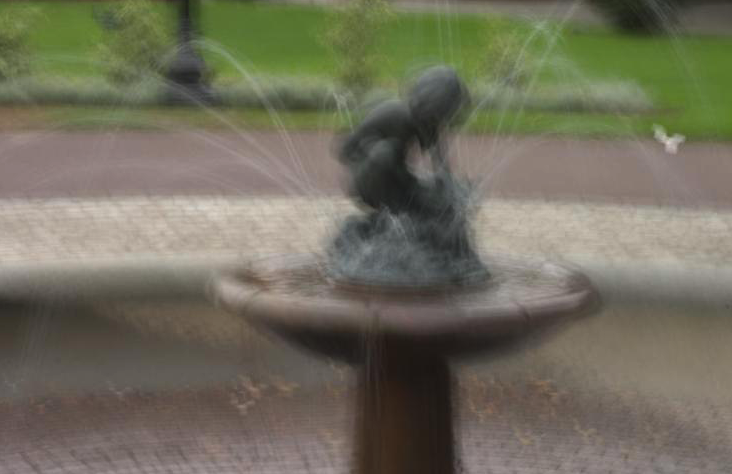
\includegraphics[width=240pt]{img/img-000.png}
    \end{center}
\end{frame}
\begin{frame}
    \frametitle{...this is how standard software solves it...}
    \begin{center}
        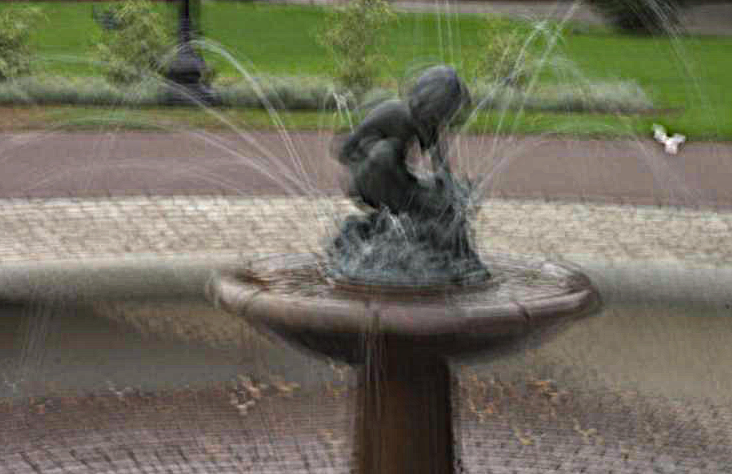
\includegraphics[width=240pt]{img/img-001.png}
    \end{center}
\end{frame}
\begin{frame}
    \frametitle{...and this is how we will solve it}
    \begin{center}
        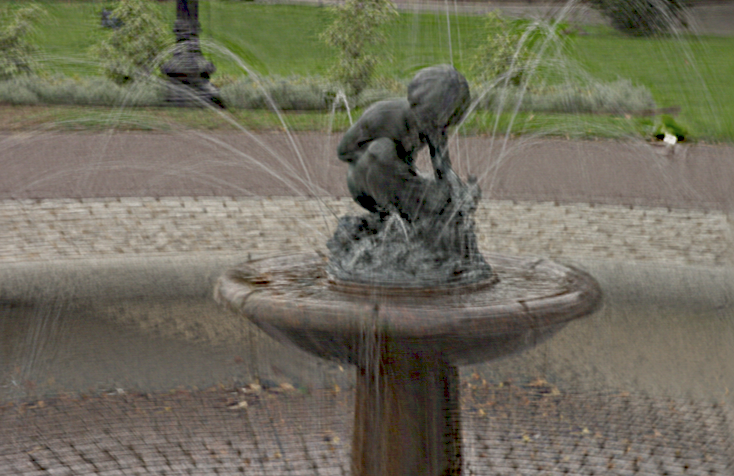
\includegraphics[width=240pt]{img/img-002.png}
    \end{center}
\end{frame}

\begin{frame}
    \frametitle{Assumptions}
    \begin{itemize}
            \item No significant parallax
            \item Any image-plane rotation of camera is small
            \item No parts of the scene are moving relative to one another
    \end{itemize}
\end{frame}
\begin{frame}
    \frametitle{Image model}
    \begin{center}
        \begin{align}
            \boldsymbol{B} &= \boldsymbol{K}\otimes\boldsymbol{L} + \boldsymbol{N}  \\
            \boldsymbol{N} &\propto \mathcal{N}(0, \sigma^2)
    \end{align}
        $\boldsymbol{B}$ is a blurred input image\\$\boldsymbol{K}$ - blur kernel\\$\boldsymbol{L}$ - true image\\$\boldsymbol{N}$ - noise
    \end{center}
\end{frame}
\begin{frame}
    \frametitle{Distribution of gradients of natural, non-blurred images}
    \begin{center}
        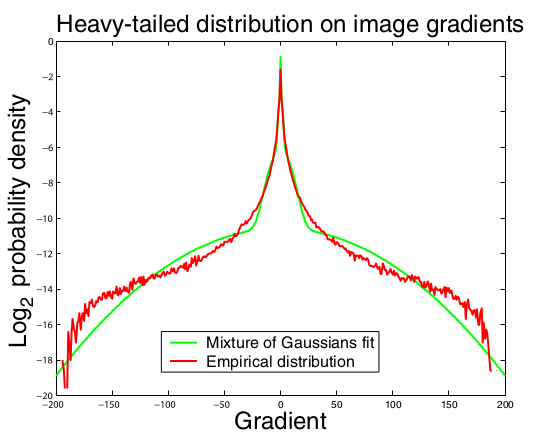
\includegraphics[width=240pt]{img/img-distr.png}
    \end{center}
\end{frame}
\begin{frame}
    \frametitle{A priori assumptions about images}
    \begin{itemize}
        \item Prior $p(\nabla P)$ is a mixture of $C$ zero-mean Gaussians (with variance $v_c$ and weight $\pi_c$)
        \item Prior $p(K)$ is a mixture of $D$ exponential distributions (with scale factors $\lambda_d$ and weights $\pi_d$).
            It encourages zero values in the kernel, and requires all entries to be positive.
    \end{itemize}
\end{frame}
\begin{frame}
    \frametitle{Algorithm}
    User supplies:
    \begin{itemize}
        \item Blurred image $\boldsymbol{B}$
        \item A rectangular patch $\boldsymbol{P}$ within the $\boldsymbol{B}$
        \item An upper bound on the size of $\boldsymbol{K}$
        \item Initial guess on the orientation of $\boldsymbol{K}$
    \end{itemize}
    We convert $\boldsymbol{P}$ to linear color space and grayscale.
\end{frame}
\begin{frame}
    \frametitle{Estimating blur kernel}
    Given the grayscale blurred patch $\boldsymbol{P}$, we estimate $\boldsymbol{K}$ and the la-
    tent patch image $\boldsymbol{L_p}$ by finding the values with highest probability, guided
    by a prior on the statistics of $\boldsymbol{L}$.
    \pause
    \\So posterior distribution will be:
    \begin{align*}
        p(\boldsymbol{K}, \nabla\boldsymbol{L_p}|\nabla\boldsymbol{P})
        &\propto p(\nabla\boldsymbol{P}|\boldsymbol{K}, \nabla\boldsymbol{L_p})p(\boldsymbol{K})p(\nabla\boldsymbol{L_p}) \\
        = &\prod_{i} \mathcal{N}(\nable\boldsymbol{P}(i)|(\boldsymbol{K}\otimes\nabla\boldsymbol{L_p}(i)), \sigma^2) \\
          &\prod_{i}\sum_{c=1}^{C} \pi_c \mathcal{N}(\nabla\boldsymbol{L_p}(i)|0,v_c) \\
          &\prod_{j}\sum_{d=1}^{D} \pi_d exp(\boldsymbol{K}_j|\lambda_d)
    \end{align*}
\end{frame}

\begin{frame}
    \frametitle{Solution}
    A straightforward approach to deconvolution is to solve for the maximum a-posteriori (MAP) solution.\\
    \pause
    \begin{center}
    {\huge It doesn't work.}\\
\end{center}
    \pause
    \begin{itemize}
        \item MAP objective function attempts to minimize all gradients (even large ones)
        \item Whereas we expect natural images to have some large gradients.
        \item The algorithm yields a two-tone image (virtually all gradients are zero)
        \item When we reduce the noise variance then we have no deblurring
    \end{itemize}
\end{frame}
\begin{frame}
    \frametitle{Solution \#2}
    Approximate the full posterior distribution $p(\boldsymbol{K}, \nabla\boldsymbol{L_p}|\nabla\boldsymbol{P})$, then compute the kernel $\boldsymbol{K}$ with \textbf{maximum marginal probability}.
    This method selects a kernel that is most likely with respect to the
    distribution of possible latent images, thus avoiding the overfitting that can occur when selecting a
single "best" estimate of the image. I won't show here details of the algorithm.
\end{frame}
\begin{frame}
    \frametitle{Multi-scale approach}
    \begin{itemize}
            \item Previous section is subject to local minima, particularly for large blur kernels
            \item Hence, we perform estimation in a coarse-to-fine manner,
                starting with a 3x3 kernel.
            \item Initial kernel is picked by user from 2 possibilities: vertical or horizontal line.
            \item Initial estimate for the $\nabla\boldsymbol{L_p}$ is produced by running the inference scheme, while holding K fixed
            \item Then we work back up, upsampling $\boldsymbol{K}$ and $\nabla\boldsymbol{L_p}$ from previous pass to use as initialization for inference at current scale.
    \end{itemize}
\end{frame}

\begin{frame}
    \frametitle{Image reconstruction}
    \begin{itemize}
        \item Standard non-blind deconvolution methods produce unacceptable levels of artifacts.
        \item Inferring whole $\nable\boldsymbol{B}$, while holding $\boldsymbol{K}$ fixed and then using Poisson image reconstruction was no better than previous attempt
        \item In the end Richardson-Lucy deconvolution algorithm gave the best results
    \end{itemize}
\end{frame}
\begin{frame}[plain]
    \begin{center}
    {\Huge Results}
    \end{center}
\end{frame}
\begin{frame}[plain]
    \begin{center}
        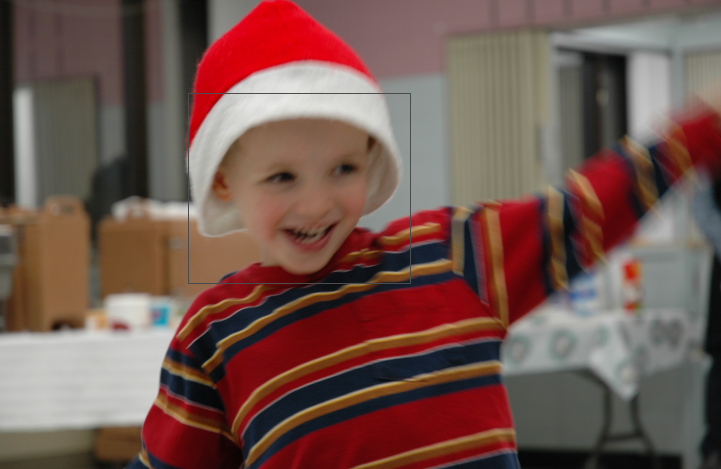
\includegraphics[width=240pt]{img/img-028.png}
    \end{center}
\end{frame}
\begin{frame}[plain]
    \begin{center}
        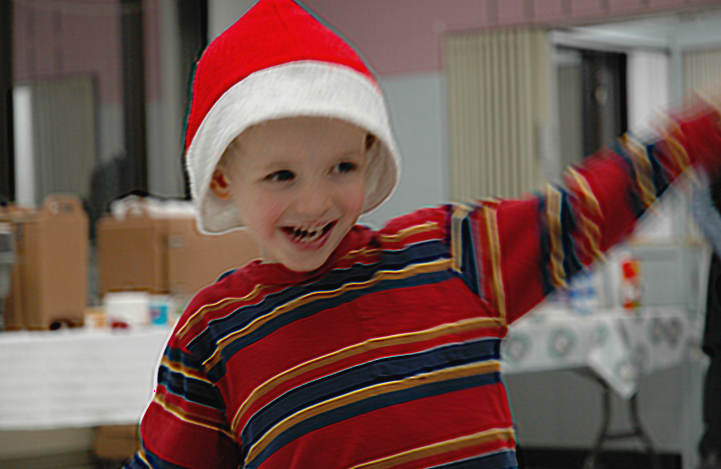
\includegraphics[width=240pt]{img/img-029.png}
    \end{center}
\end{frame}
\begin{frame}[plain]
    \begin{center}
        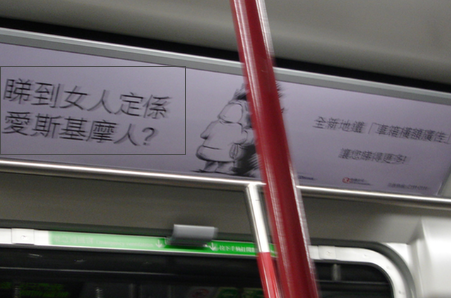
\includegraphics[width=240pt]{img/img-025.png}
    \end{center}
\end{frame}
\begin{frame}[plain]
    \begin{center}
        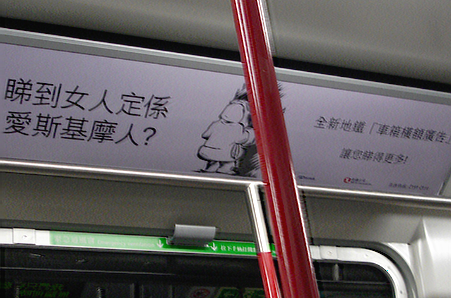
\includegraphics[width=240pt]{img/img-026.png}
    \end{center}
\end{frame}
\begin{frame}[plain]
    \begin{center}
        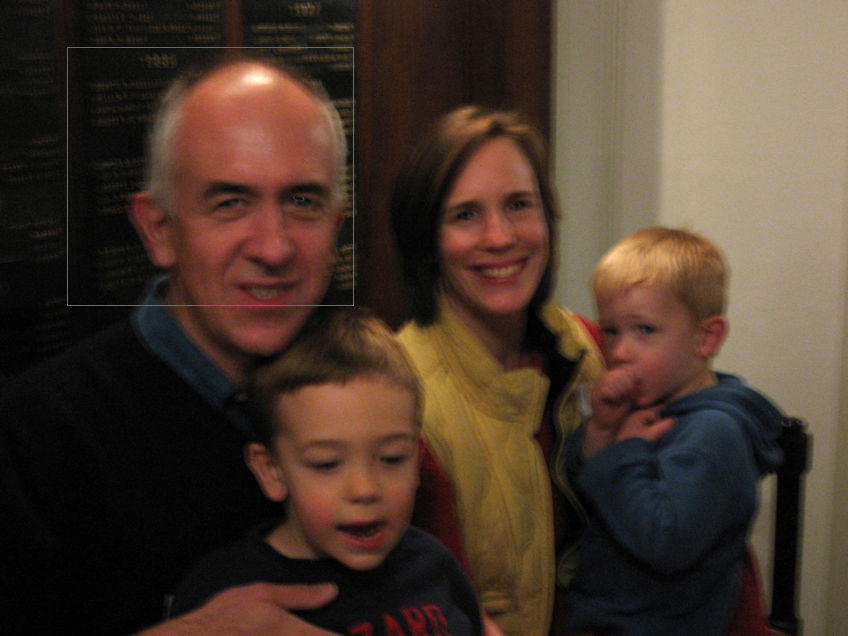
\includegraphics[width=240pt]{img/img-031.png}
    \end{center}
\end{frame}
\begin{frame}[plain]
    \begin{center}
        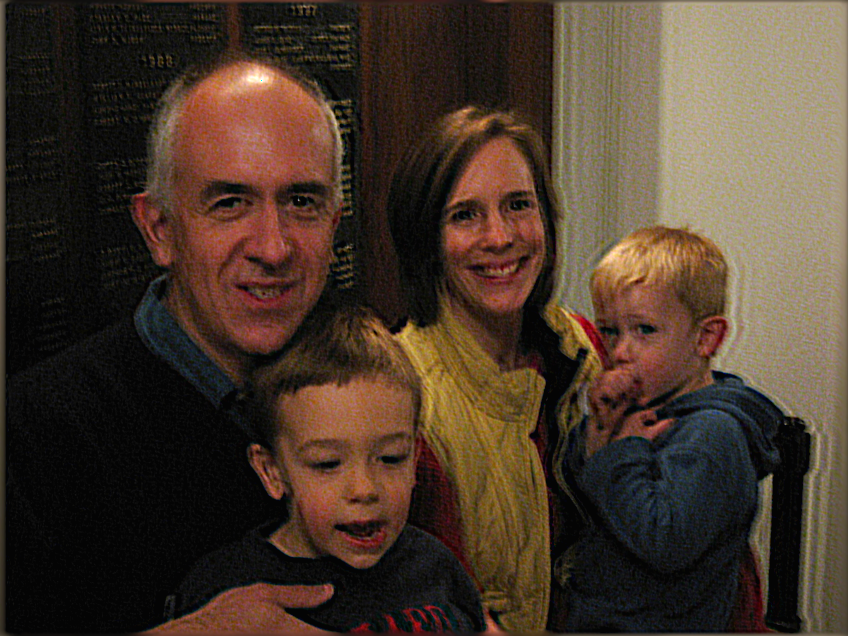
\includegraphics[width=240pt]{img/img-032.png}
    \end{center}
\end{frame}
\end{document}
